%--------------------Base----------------------------%
\documentclass[a4paper]{article}
\usepackage[utf8]{inputenc}
\usepackage[T1]{fontenc}
\usepackage[english]{babel}
\usepackage[autostyle=true]{csquotes} % Required to generate language-dependent quotes in the bibliography
\usepackage{geometry}
\geometry{
	paper=a4paper, % Change to letterpaper for US letter
	inner=2.5cm, % Inner margin
	outer=2.5cm, % Outer margin
	top=2.5cm, % Top margin
	bottom=2.5cm, % Bottom margin
	%showframe,% show how the type block is set on the page
}
\usepackage{booktabs}
\usepackage[dvipsnames]{xcolor}  
\usepackage{color}
\usepackage{setspace}
\onehalfspacing
\usepackage[colorlinks=true,citecolor=Maroon]{hyperref}

\usepackage{pdflscape}
%---------------------MATH----------------------------%
\usepackage{amsmath}
\usepackage{amssymb}
\usepackage{dsfont}
\usepackage{amsthm}
\usepackage{mathtools}
\theoremstyle{plain}
\newtheorem{assumption}{Assumption}
\newtheorem{proposition}{Proposition}
\newtheorem{definition}{Definition}
\newtheorem{lemma}{Lemma}
\allowdisplaybreaks
%---------------------FONT----------------------------%
\usepackage{microtype}
\usepackage{charter}
%-------------------GRAPHIC ---------------------%
\usepackage{float}
\usepackage{graphicx}
\graphicspath{{../figures_03_2020/}}
\usepackage{tikz}
\usepackage{pgfplots}
\pgfplotsset{compat=1.5}

%-------------------BIBLIOGRAPHY--------------------%
\usepackage{natbib}

%---------------THESIS INFORMATION-----------------%

\title{\textbf{Fluctuations in a Dual Labor Market}}
\author{Normann Rion\footnote{Ecole Normale Supérieure and Paris School of Economics. E-mail: \href{mailto:normann.rion@psemail.eu}{\texttt{normann.rion@psemail.eu}}}}
\date{\today}

\begin{document}

\maketitle

%\begin{abstract}
%I build a New-Keynesian DSGE model with a dual labor market. Firms and workers meet through a matching technology à-la Diamond-Mortensen-Pissarides and face a trade-off between productivity and flexibility at the hiring stage. Open-ended contracts are more productive than fixed-term contracts, but they embed a firing tax. Importantly, the share of fixed-term contracts in job creations fluctuates endogenously, which enables to assess the resort to temporary contracts along the cycle and its response to different shocks. I use classic Bayesian procedures with data from the Euro Area to estimate the model. The latter replicates well the counter-cyclicality of the share of temporary contracts in job creation, as well as more classic features of a dual labor market. The agents react to shocks essentially through the job creation margin and the contractual composition of the hired workers. Moreover, a general-equilibrium effect arises ; the substitution between temporary and permanent contracts at the hiring stage influences the job seekers' stock, which in turn impacts the job creation margins. Inflation dynamics depend on newly hired workers' productivity and contractual composition. Reforms in employment protection legislation entail small persistent movements in inflation.\\
%\textbf{JEL Classification: J42, J64, E31, E32 } \\
%\textbf{Keywords: Fixed-term contracts, Employment protection, New Keynesian model} 
%\end{abstract}

%\section*{Introduction}

In the past decades, fixed-term employment has grown in importance on European labor markets. In France, for example, temporary contracts represented 5 \% of employed workers in the 80s, while it fluctuates around 15\% today. Around 80 \% of job creation occurs through temporary contracts nowadays, most of them with a stipulated duration of less than one month\footnote{See \citet{fontaine2016cdd} for an overview of the situation in European countries}. Fixed-term employment serves as a buffer against immediate workload fluctuations\footnote{See \citet{doi:10.1111/iere.12167} } and, to this extent, shares the time scale of conventional monetary policy. I estimate a New-Keynesian DSGE model with a dual labor market using Euro-area data to study the interaction between these two.

The contribution is threefold. First of all, the model is able to account for the contractual composition of hires and its fluctuations. The strong counter-cylicality of the share of temporary contracts in job creation is well rendered, among other moments characterizing a dual labor market. Secondly, the possibility to substitute temporary contracts and permanent contracts at the hiring stage plays an important role on impact. This initial substitution effect on the composition of job creation impacts the number of job seekers, which in turn influences the thickness of job creation flows. There is a direct link between fluctuations in composition of job creation and fluctuations in the quantity of job creation. Finally, I find that the newly hired workers' contractual composition and productivity intervene in inflation dynamics. Marginal and transitory reforms on employment protection legislation, which are frequent in the Euro Area\footnote{\citet{fontaine2016cdd} state that reforms are actually frequent and often marginal in Western and Southern Europe. Between 2005 and 2013, they count 17 employment protection legislation reforms in France, 49 in Italy, 38 in Spain, 23 in Greece and 17 in Portugal}, generate small and persistent movements in inflation.

The literature is scarce when it comes to consider both a truly endogenous choice between open-ended and fixed-term contracts and fluctuations in a dual labor market. The main references when it comes to study cycles with a dual labor market are the pioneering papers of \citet{sala2009flexibility}, \citet{RePEc:bde:journl:y:2010:i:04:n:04} and \citet{SJOE:SJOE1715}. These models either assume that job creation only occurs through temporary contracts, or the share of temporary contracts is constant and exogenously set. However, \citet{shimer2005cyclical} demonstrates the importance of job creation flows in the understanding of unemployment fluctuations. Moreover, given the overwhelming prominence of temporary contracts in job creation flows, the contractual composition of hires needs to be considered from a policy perspective.

In this paper, firms and workers meet as in the classic \citet{mortensen1994job} ; firms maintain vacancies while workers search for a job. When a firm and a worker meet, they draw a productivity and choose between a fixed-term contract and an open-ended contract accordingly. The resulting match then faces i.i.d shocks on its productivity. I assume that open-ended contracts are more productive than fixed-term contracts. Open-ended contracts embed a firing cost in case of endogenous separation, whereas temporary contracts stipulate an exogenous short duration without a separation cost. As a result, fixed-term contracts enable a quick and costless split in the doldrums. This productivity-flexibility trade-off is highlighted in several papers. \citet{cao2010fixed} show that highly productive workers are offered permanent contracts, because temporary workers have an incentive to search on the job, which depletes their productivity. \citet{10.2307/20485287}, as for them, introduce temporary contracts, which are less productive than permanent contracts by assumption, in firms with a decreasing-return-to-scale technology. As a result, firms hire permanent contracts until the productivity gains are offset by the expected losses from costly separations, and hire temporary contracts beyond that point. \citet{rion:halshs-02331887} is the closest paper when it comes to the economic schemes at the hiring stage.

The assumption of an existing contractual productivity wedge is fundamental and deserves justification. Temporary workers are likely to undergo successions of short employment periods and long unemployment spans \citep{fontaine2016cdd}. \citet{pissarides1992loss} shows that the latter reduce concerned  workers' skills. Moreover, fixed-term positions are mainly filled by low-skilled or unexperienced workers \citep{fontaine2016cdd}, who benefit less from on-the-job training \citep{doi:10.1111/1467-8543.00106,10.1162/154247604323068041,Albert2005,10.1093/esr/jcs011}.

The study of nominal rigidities along with fluctuations in frictional labor markets constitutes a leafy literature\footnote{See, among many others,\citet{gertler2008estimated}, \citet{trigari2009equilibrium} and \citet{christiano2016unemployment} among others}, where dualism has never been considered, as far as I know.  For the sake of comparability, I stick to \citet{thomas2009labor} when it comes to the New-Keynesian block. They introduce employment protection legislation in a Mortensen-Pissarides model along with nominal rigidities but the labor market only includes open-ended contracts.

The paper is organized as follows. Section 2 presents the model. Section 3 exposes the calibration and estimation procedure. Section 4 displays the main results of our analysis. Section 5 concludes.  
%\input{literature}
\section{Model}

The model follows a discrete timing and embeds 4 types of agents; the households, the firms, the fiscal authority and the central bank. Households can be unemployed or employed through a fixed-term or an open-ended contract. Three types of firms coexist. Perfectly competitive firms produce the final good valued by households for consumption and investment. Final good producers aggregate the differentiated goods produced by the retailers. The latter retailers are in monopolistic competition and transform the homogeneous intermediate good into a differentiated retail good. Intermediate firms produce the associated intermediate good and experience perfect competition. These intermediate firms use labor as their only input. I now describe the behavior of different types of agents in more detail.

\subsection{Households}

Households are identical and constitute a continuum represented  by the interval $(0,1)$. They can be employed under a fixed-term or an open-ended contract, or unemployed. They earn wages or unemployment benefits accordingly. Households also hold firms, consume the homogeneous good produced by final good firms, save using one-period nominal bonds, earn interests on their savings and pay lump-sum taxes. Hence, I assume that taxes do not distort the choice of households over consumption and investment. I do not consider the interplay between payroll taxes and labor market dualism.

If households are identical \emph{ex ante}, their different employment histories make them heterogeneous \emph{ex post}. How labor market dualism impacts the consumption and saving behavior of households is beyond the scope of this paper. As \citet{merz1995search} and \citet{andolfatto1996business} first did, I assume that households pool revenues and that capital markets are perfect. Thereby, I rule out the complication heterogeneity brings on. Households share equal consumption and investments. This assumption is not innocuous: unemployed, open-ended and fixed-term workers have different borrowing constraints and \citet{10.2307/43551457} shows that assets shape the search behavior. I leave these issues for future research. 

The household's program boils down to

\begin{align*}
&\max_{\left\{c_t, B_{t+1} \right\}_{t=0}^{+\infty}} \mathbb{E}_0 \sum_{t = 0}^{+\infty} \beta^t u\left(c_t\right)\\
&\text{s.t} \quad c_t + \frac{B_{t+1}}{P_t} = R_{t-1} \frac{B_{t}}{P_t} + \overline{w_t^p} n_t^p + \overline{w_t^f} n_t^f + \rho^b \overline{w_t} u_t + \Pi_t - \tau_t
\end{align*}

$C_t$ marks down consumption. $B_{t}$ is the amount of nominal bond holdings at the beginning of period $t$, with the associated nominal interest rate $R_t$ between $t$ and $t+1$. $\overline{w_t^p}$, $\overline{w_t^f}$ and $\overline{w_t}$ denote respectively the average real wages for open-ended jobs, temporary jobs and all workers. $\rho^b$ denotes the replacement rate of unemployment benefits over the average wage. $n_t^p$ is the aggregate open-ended employment and $n_t^f$ denotes its fixed-term counterpart. $u_t$ marks down the measure of unemployed households. Firms transfer their profits to households through $\Pi_t$, while the government taxes $\tau_t$ to finance the payment of unemployment benefits.

The first order conditions with respect to $c_t$ and $B_{t+1}$ lead to the following Euler equation

\begin{equation}
u' \left( c_t \right) = \beta \mathbb{E}_t \left[ R_{t} \frac{P_t}{P_{t+1}} u' \left( c_{t+1} \right) \right] \label{eq:euler_eq}\\
\end{equation}

As households own firms, the firms' discount factor is $\beta_{t,s} = \beta^{s-t} u' \left( c_s \right) / u' \left( c_t \right)$.

\subsection{Final good firms}

Final good firms are identical and compete to produce the good consumed by households. They use a Dixit-Stiglitz aggregator as technology to put together retail goods and produce $Y_t$.

\begin{equation}
Y_t = \left( \int_{0}^{1} Y_{i,t}^{\frac{\epsilon - 1}{\epsilon_t}} di \right)^{\frac{\epsilon}{\epsilon} - 1} \label{con_fin}
\end{equation}

where $\epsilon$ is the elasticity of substitution between retail goods.

The firm takes as given the price of the retail goods $P_{i,t}$ and the price of the final good $P_t$ and maximizes its profits with respect to the components of its input $\left\{Y_{i,t}\right\}_{i\in(0,1)}$ under the constraint \eqref{con_fin}. The program of the final good firm boils down to

\begin{align*}
&\max_{\left\{Y_{i,t}\right\}_{i\in[0,1]}} P_t Y_t - \int_{0}^{1} P_{i,t} Y_{i,t} di\\
&\text{subject to \eqref{con_fin}}
\end{align*}

The subsequent first order condition provides an expression for the demand of the retail good $i$

\begin{equation}
Y_{i,t} = \left( \frac{P_{i,t}}{P_t} \right)^{-\epsilon} Y_t \label{eq:ret_dem}
\end{equation}

\subsection{Retailers}

Retailers buy goods from intermediate firms and sell the obtained production to final good producer\footnote{At this step, it is possible to introduce capital to extend the model.}. They are in monopolistic competition and lie on the interval $(0,1)$. Retailers accomplish the one-to-one transformation of the intermediate good into a retail good. Denoting $X_{i,t}$ the retailer's input in the intermediate good, the production technology writes

\begin{equation*}
Y_{i,t} = X_{i,t}
\end{equation*}

As a result, retailers face a real marginal cost that equals the relative price of the intermediate good $\phi_t$. I assume that retailers adjust prices as \citet{calvo1983staggered} describe.

\begin{align*}
P_{i,t} = \left\{ \begin{array}{ll}
P_{i,t-1} & \text{ with probability } \psi\\
P_{i,t}^* & \text{ with probability } 1-\psi\\
\end{array}
\right.
\end{align*}

A fraction $\psi$ of retailers is able to adjust its prices to the optimal value $P_{i,t}^*$, whereas the  remaining retailers stick to their former prices. There is no indexation of non-adjusted princes on inflation in this model. The price-setting retailer $i$ at period $t$ has the following program

\begin{align*}
&\max_{P_{i,t}^*} \mathbb{E}_{t} \sum_{T = t}^{+\infty} \beta_{t,T} \psi^{T-t} \left( \frac{P_{i,t}^*}{P_T} - \phi_{T} \right) Y_{i,T} \\
&\text{ subject to } Y_{i,T} = \left( \frac{P_{i,t}^*}{P_T} \right)^{-\epsilon_T} Y_T
\end{align*}

This leads to the following first order condition

\begin{equation}
\mathbb{E}_{t} \sum_{T = t}^{+\infty} \beta_{t,T} \psi^{T-t} P_T^{\epsilon_T} Y_T \left( \frac{P_{i,t}^*}{P_T} - \mu \phi_T \right) = 0 \label{eq:price_eq}
\end{equation}

where $\mu = \epsilon /(\epsilon-1)$ is the mark-up of retailers.

\subsection{Intermediate good firms and the labor market}

Intermediate-good firms use labor as input. They can employ one worker or maintain one vacancy. Workers can be unemployed or employed under a fixed-term or an open-ended contract. They are identical. There is no on-the-job search, which implies that only unemployed workers search for a job. When a firm and a worker meet, the idiosyncratic productivity of the match $z$ is revealed. I assume that idiosyncratic productivity is i.i.d across time and drawn from a distribution with cumulative distribution function $G$. I reluctantly make this assumption for the sake of simplicity. With persistent idiosyncratic productivity, the computation of the equilibrium requires keeping track of the productivity distribution of matches as a state variable. Since the literature considering cycles and dual labor market is in early stages, I prefer to leave the distributional issues for future research. 

The number of firm-worker contacts per period is $m(e,v)$, where $e$ is the number of job-seekers and $v$ is the number of vacancies. A classic measure of the matching activity is the labor market tightness $\theta =  v/e$. The matching function $m$ has constant returns to scale, which enables the definition of the firm-worker meeting probability $p(\theta)$ on the job seekers' side and its counterpart $q(\theta)$ on the firms' side.

\begin{align*}
q &= \frac{m\left(e,v\right)}{v} = m \left( \theta^{-1}, 1\right)\\
p &= \frac{m\left(e,v\right)}{e} = m \left( 1, \theta\right) = \theta q(\theta)\\
\end{align*}

$p$ is increasing in labor market tightness, whereas $q$ is decreasing in labor market tightness. Note that the meeting probabilities are not the classic job-finding and vacancy-filling probabilities. A firm-worker meeting does not lead to a production if the idiosyncratic productivity is too low.  

The timing in the economy is summed up in Figure \ref{fig:timing}. At the beginning of the period, agents learn the value of shocks and firms manage their workforce accordingly. They lay off poorly productive workers and post vacancies. Next, new matches are revealed. Workers fired in the current period are able to participate to the present meeting round. Hence, I avoid understating labor market flows as most fixed-term contracts last less than a quarter: fixed-term jobs last 1.5 months on average in France \citep{dares062018}. Finally, production is carried out, firms pay for wages and firing costs, households consume, and the period ends. 

\begin{figure}[H]
\begin{center}
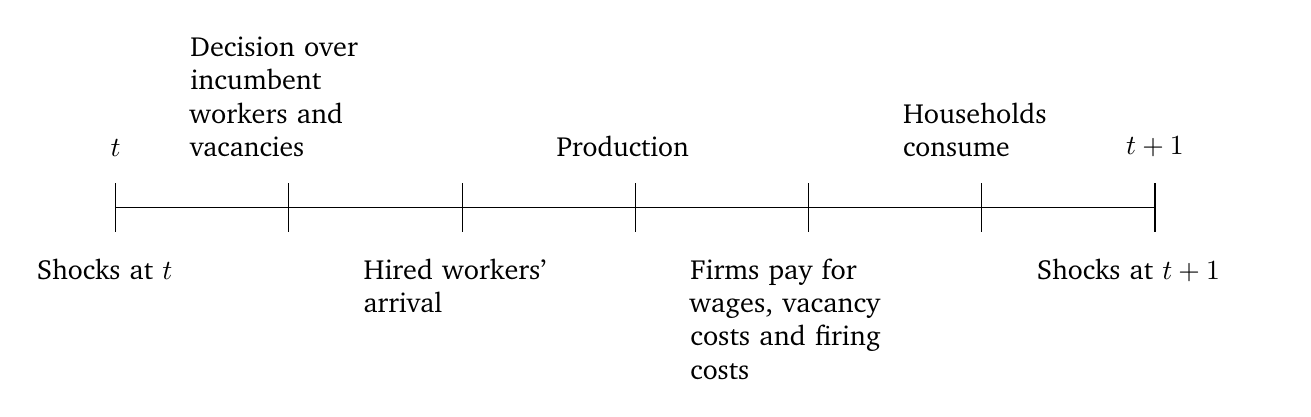
\begin{tikzpicture}[scale = 0.88]
%draw horizontal line
\draw (0cm,0cm) -- (15cm,0cm);
draw vertical lines
\foreach \x in {0, 2.5, 5, 7.5, 10, 12.5, 15}{
   \draw (\x,10pt) -- (\x,-10pt);
}
\draw (0,0) node[below=15pt, text width=2cm] {Shocks at $t$} node[above=15pt] {$t$};
\draw (2.5,0) node[above=15 pt, text width=2.5cm] {Decision over incumbent workers and vacancies};
\draw (5,0) node[below=15pt, text width=2.5cm] {Hired workers' arrival};
\draw (7.5,0) node[above=15pt, text width=2cm] {Production};
\draw (10,0) node[below=15pt, text width=3cm] {Firms pay for wages, vacancy costs and firing costs};
\draw (12.5,0) node[above=15pt, text width=2cm] {Households consume};
\draw (15,0) node[below=15pt, text width=3cm] {Shocks at $t+1$} node[above=15pt] {$t+1$};
\end{tikzpicture}
\end{center}
\label{fig:timing}
\caption{The timing of the economy}
\end{figure}

\paragraph{Vacancies} I depart from the literature when it comes to job creation. \citet{sala2009flexibility} assumes that job creation occurs through fixed-term contracts only; open-ended jobs all come from converted fixed-term jobs, which is counterfactual. As \citet{CAHUC200263} first did, \citet{SJOE:SJOE1715} assume that new matches face hiring restrictions. Firms are allowed to hire either through an open-ended or a fixed-term contract according to an exogenous probability. Otherwise, all hires would take place through fixed-term contracts. As roughly 20\% of hires are open-ended in France, different reasons than legal constraints on fixed-term hires explain open-ended hires.

Thereby, I assume that no constraints bind job creation. When paired with a worker, firms hire through a fixed-term contract or through an open-ended contract. They can also return searching for a worker and get the chance to be matched with another one on the next period. The present discounted value of a vacancy $V_t$ bears witness of these different options:

\begin{equation} \label{eq:def_v}
V_t = - \gamma + q \left( \theta_{t} \right) \int max \left[ J_{t}^{0,p} \left( z \right) , J_{t}^{f} \left( z \right) ,  \mathbb{E}_{t} \beta_{t,t+1} V_{t+1} \right] dG(z)
\end{equation}

where $\gamma$ is the cost of a vacancy, $J_{t}^{0,p}$ is the firm's surplus with a new open-ended match and $J_t^{0,f}$ is the firm's surplus with a new fixed-term match. The counterpart of these surpluses for continuing open-ended matches and continuing fixed-term matches are $J_{t}^{p}$ and $J_t^{f}$. The associated surpluses of workers are denoted $W$, while the total surpluses are denoted $S$. 

\paragraph{Surplus sharing}

I assume that wages are set each period by Nash bargaining. It is not realistic considering the evidence supporting rigidity in wages. In addition, wage flexibility seems inconsistent with the stickiness of retailers' prices. Still, I leave rigid wages for future research. Tractability motivates the use of Nash bargaining. It makes hiring and firing decisions jointly efficient and only dependent on the total surplus of a match. Denoting $\eta$ the worker's share of the match surplus, the sharing rules write

\begin{align}
&W_t^p \left( z_t \right) = \eta S_t^p \left( z_t \right) \label{eq:nash_p}\\
&W_t^{0,p} \left( z_t \right) = \eta S_t^{0,p} \left( z_t \right) \label{eq:nash_0p}\\
&W_t^f \left( z_t \right) = \eta S_t^f \left( z_t \right) \label{eq:nash_f}
\end{align}

Total surpluses verify

\begin{align}
S_t^p \left( z_t \right) &= J_t^p \left( z_t \right) - \left( V_t - F_t \right) + W_t^p \left( z_t \right) - U_t \label{eq:def_sp}\\
S_t^{0,p} \left( z_t \right) &= J_t^{0,p} \left( z_t \right) - V_t + W_t^{0,p} \left( z_t \right) - U_t \label{eq:def_s0p}\\
S_t^{f} \left( z_t \right) &= J_t^{f} \left( z_t \right) - V_t + W_t^{f} \left( z_t \right) - U_t \label{eq:def_sf}
\end{align}

where $U_t$ is the value of unemployment at the beginning of period $t$. The outside option of workers includes taking part in current period's market trades and take the unemployment benefit if no beneficial meeting occurred.

\begin{align}
U_t &= p\left( \theta_t \right) \int \max \left( W_t^{0,p} (z), W_t^f (z), U_t^0 \right) dG(z) + \left( 1 - p\left( \theta_t \right) \right)U_t^0 \label{eq:U} \\
U_t^0 &= b_t + \mathbb{E}_t \beta_{t, t+1} U_{t+1} 
\end{align}

where $b_t = \rho^b \overline{w_t} + h$ is the unemployed's flow of utility. It includes unemployment benefits as well as home production $h$. 

In \eqref{eq:def_sp}-\eqref{eq:def_sf}, note that the surplus of incumbent open-ended matches includes firing costs, while the one of new open-ended workers does not. In case of disagreement during wage bargaining, a newly paired worker goes back to the pool of job seekers and the firm does not pay firing costs. That way, I do not overstate the role of firing costs.

Now, I describe the open-ended and the fixed-term contract and the associated surpluses.

\paragraph{Open-ended contracts}

A continuing open-ended contract delivers the wage $w_{t}^{p}$ and stipulates a firing tax $F_t$. An open-ended match may separate with the exogenous probability $s$. In this case, the separation bears no cost. Otherwise, the firm chooses whether it keeps or lays off the worker regarding the idiosyncratic productivity of the match. An endogenous separation entails the payment of the firing cost and the opening of a new vacancy. Hence, a firm with an incumbent open-ended worker has the following surplus

\begin{align} \label{eq:def_jp}
J_t^p \left( z_{t} \right) = \phi_t A_t z_{t} - w_{t}^{p} \left( z_t \right) + \mathbb{E}_{t} \beta_{t,t+1} \left\{ (1-s) \int \max \left[ J_{t+1}^{p} \left( z \right), V_{t+1} - F_{t+1} \right] dG(z) + s V_{t+1} \right\}
\end{align}

An incumbent open-ended worker earns a wage and may leave with probability $s$. If he does not, he faces a productivity shock and the match may split if the latter shock is adverse enough. Laid-off or quitting workers go back to the job seekers' pool immediately and are therefore eligible to participate to the current's period firm-worker meetings. Otherwise, the match goes on.

\begin{equation} \label{eq:def_wp}
W_t^p \left( z_t \right) = w_{t}^{p} \left( z_t \right) + \mathbb{E}_{t} \beta_{t,t+1} \left\{ (1-s) \int \max \left[ W_{t+1}^p ( z ), U_{t+1} \right]  dG(z) + s U_{t+1} \right\}
\end{equation}

New open-ended workers have a different wage function $w_t^{0,p}$: their outside option does not include the payment of the firing cost in case of disagreement during the wage bargaining and the possibility to search for a new job in case of disagreement. After one-period, if there is no separation, a wage renegotiation occurs because idiosyncratic productivity changed. The firm pays firing costs if an endogenous split occurs. Otherwise, the surplus of incumbent open-ended contracts weighs in. 

\begin{align} \label{eq:def_j0p} 
J_t^{0,p} \left( z_{t} \right) &= \phi_t A_t z_{t} - w_{t}^{0,p} \left( z_t \right) + \mathbb{E}_{t} \beta_{t,t+1} (1-s) \left\{ \int_{z_{t+1}^p}^{+\infty} J_{t+1}^{p} \left( z \right) dG(z) - G\left(z_{t+1}^p\right) F_{t+1} + s V_{t+1} \right\}\\
W_t^{0,p} \left( z_t \right) &= w_{t}^{0,p} \left( z_t \right) + \mathbb{E}_{t} \beta_{t,t+1} \left\{ (1-s) \int \max \left( W_{t+1}^p ( z ), U_{t+1} \right) dG(z) + s U_{t+1} \right\}
\end{align} 

\paragraph{Fixed-term contracts} A fixed-term contract stipulates the wage function $w_{t}^{f}$. Fixed-term matches split with the exogenous probability $\delta$. I assume that fixed-term contracts yield a lower productivity than open-ended matches with a factor $\rho < 1$. I discuss this assumption in detail below. Firms value the immediate production net of the wage. As for the continuation value, it simply embeds the possibility of an exogenous separation shock.

\begin{equation} \label{eq:def_jf}
J_{t}^f \left( z_t \right) = \rho A_t z_t \phi_t - w_{t}^{f} \left( z_t \right) + \mathbb{E}_{t} \beta_{t,t+1} \left\{ \left( 1-\delta \right)  \int J_{t+1}^{f} \left( z \right) dG(z) + \delta V_{t+1} \right\}
\end{equation}

Fixed-term workers immediately value their wage. In case of separation, they can immediately indulge in labor market trades.

\begin{equation} \label{eq:def_wf}
W_{t}^f \left( z_t \right) = w_{t}^{f} \left( z_t \right) + \mathbb{E}_{t} \beta_{t,t+1} \left\{ \left( 1-\delta \right)  \int W_{t+1}^{f} \left( z \right) dG(z) + \delta U_{t+1} \right\}
\end{equation}

Using the different definitions of the firms' and the workers' surpluses, the total surpluses write\footnote{Detailed calculations are available in Appendix \ref{sec:nb_surplus}}

\begin{align}
\begin{split} \label{eq:sp}
S_t^p \left( z_t \right) &= A_t z_t \phi_t - b - \frac{\eta \gamma \theta_{t}}{1-\eta} + F_t - \mathbb{E}_t \beta_{t,t+1} (1-s) F_{t+1} \\
&+ \mathbb{E}_t  \beta_{t,t+1} (1-s) \int \max \left( S_{t+1}^p \left( z \right), 0 \right) dG(z)
\end{split}\\
S_t^{0,p} \left( z_t \right) &= S_t^p \left( z_t \right) - F_t\label{eq:s0p}\\
S_t^f \left( z_t \right) &= \rho A_t z_t \phi_t - b - \frac{\eta \gamma \theta_{t}}{1-\eta} + \rho \mathbb{E}_t \beta_{t,t+1} (1-\delta) \int S_{t+1}^f ( z ) dG(z)\label{eq:sf}
\end{align}

As intended, the surplus of continuing open-ended workers includes the firing cost in case of endogenous separation. This bolsters his threat point in Nash bargaining and pushes up his wage. The new open-ended workers does not benefit from this effect since a failure in the bargaining process does not entail the payment of $F_t$. The total surplus of fixed-term workers shows the productivity gap $\rho$ in the flows and the exogenous termination of the contract in the continuation value. Fixed-term contracts hit with a job destruction shock split regardless the productivity of the match.

Using the firms' surpluses, joint surpluses and the surplus sharing rules, wages verify

\begin{align}
w_t^p \left( z_t \right) &= \eta \left( A_t z_t \phi_t + F_t - E_t \beta_{t,t+1} (1-s) F_{t+1} + \gamma \theta_{t} \right) + (1-\eta) b_t \label{eq:wp}\\
w_t^{0,p} \left( z_t \right) &= \eta \left( A_t z_t \phi_t - E_t \beta_{t,t+1} (1-s) F_{t+1} + \gamma \theta_{t} \right) + (1-\eta) b_t\\
w_t^f \left( z_t \right) &= \eta \left( \rho A_t z_t \phi_t + \gamma \theta_{t} \right) + (1-\eta) b_t\\
\end{align}

The new open-ended worker is penalized with higher firing costs to compensate the future gains of wages in case of continuation. Moreover, labor market tightness increases the outside option of workers through the higher probability of finding a job. Wages increase with labor market tightness.

\subsection{Job creation and job destruction}

I assume there is free entry on vacancy posting.

\begin{equation}
V_t = 0 \label{eq:free_entry}
\end{equation}

The job creation condition stems from the free-entry condition \eqref{eq:free_entry} and the Bellman equation defining the present discounted value of an unfilled vacancy \eqref{eq:def_v}. Using the Nash-sharing rules \eqref{eq:nash_0p}-\eqref{eq:nash_f}, the job creation condition becomes

\begin{align*}
\frac{\gamma}{(1-\eta) q\left( \theta_t \right)} = \int max \left[ S_t^{0,p} \left( z \right) , S_t^{f} \left( z \right), 0\right] dG(z)
\end{align*}

The choice between fixed-term and open-ended contracts lies in the comparison of joint surpluses across contracts. Notice that $\partial S_t^{0,p} / \partial z_t = A_t \phi_t A_t > \rho A_t \phi_t = \partial S_t^{f} / \partial z_t$. Thus, there exists a productivity threshold $z_t^*$ above which open-ended contracts are preferable to fixed-term ones.

\begin{align*}
S_t^{0,p} \left( z_t^* \right) = S_t^{f} \left( z_t^* \right) 
\end{align*}

As a result, job creation with \eqref{eq:def_sp_lin} and \eqref{eq:def_sf_lin}, one finds that $z_t^*$ verifies

\begin{equation}
(1-\rho) z_t^* = z_t^c - \rho z_t^f \label{eq:zs}
\end{equation}

I also define the threshold $z_t^p$ below which an incumbent open-ended match splits. Similarly, fixed-term contracts become profitable when productivity exceeds $z_t^f$. I denote $z_t^c$ the analogous threshold for new open-ended contracts.

\begin{align} \label{eq:def_zp}
&S_t^p \left( z_t^p \right) = 0 \\
\label{eq:def_zf}
&S_t^{f} \left( z_t^f \right) = 0\\ \label{eq:def_zc}
&S_t^{0,p} \left( z_t^c \right) = 0
\end{align}

Joint surpluses are linear in $z_t$. I can rewrite them using \eqref{eq:def_zp}-\eqref{eq:def_zf}. 

\begin{align}
&S_t^p (z) = A_t \phi_t \left( z - z_t^p \right) \label{eq:def_sp_lin} \\
&S_t^f (z) = \rho A_t \phi_t \left( z - z_t^f \right) \label{eq:def_sf_lin}
\end{align}

Using \eqref{eq:sp}-\eqref{eq:def_zc} and with integrations by part, equations profitability thresholds.

\begin{align} \label{eq:zp}
\begin{split}
&A_t z_t^p \phi_t + F_t - \mathbb{E}_t \beta_{t,t+1} (1-s) F_{t+1} + \mathbb{E}_t  \beta_{t,t+1} (1-s) A_{t+1} \phi_{t+1} \int_{z_{t+1}^p}^{+\infty} \left( 1 -  G(z) \right) dG(z)\\
&= b_t + \frac{\eta \gamma \theta_{t}}{1-\eta}
\end{split} \\
&A_t \phi_t z_t^c = A_t \phi_t z_t^p + F_t \label{eq:zc} \\
&\rho A_t z_t^f \phi_t + \rho \mathbb{E}_t \beta_{t,t+1} (1-\delta) A_{t+1} \phi_{t+1} \left( \mathbb{E}z - z_{t+1}^f \right) = b_t + \frac{\eta \gamma \theta_{t}}{1-\eta} \label{eq:zf}\\
\end{align}

Using these thresholds and integrations by part, I rewrite the job creation condition.

\begin{align} \label{eq:jc}
\frac{\gamma}{(1-\eta) q\left( \theta_t \right) A_t \phi_t} = \int_{\max \left[ z_t^c, z_t^* \right]}^{+\infty} \left( 1-G(z) \right) dz + \rho \int_{z_t^f}^{\max \left[ z_t^c, z_t^* \right]} \left( 1-G(z) \right) dz
\end{align}

The following proposition sums up job creation.

\begin{proposition} \label{prop:jc} Given $\left( z_t^p, z_t^c, z_t^f, z_t^* \right)$,
\begin{itemize}
\item if $z_t^* \leq z_t^f \leq z_t^c$, job creation is carried out through open-ended contracts only. it occurs when $z \geq z_t^c$ as figure \ref{fig:oe_only} shows.

\begin{figure}[H]
\centering
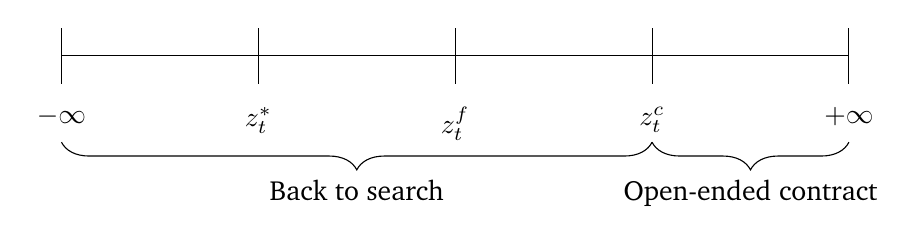
\begin{tikzpicture}[]
%draw horizontal line
\draw (0,0) -- (10cm,0);
%draw vertical lines
\foreach \x in {0,2.5,5,7.5,10}{
   \draw (\x cm, 10pt) -- (\x cm,-10pt);
}

%draw nodes
\draw (0,0) node[below=15pt,name = zbeg] {$-\infty$};
\draw (2.5cm,0) node[below=15pt,name = zs] {$z_t^*$};
\draw (5cm,0) node[below=15pt,name=  zf] { $z_t^f$};
\draw (7.5cm,0) node[below=15pt,name=  zc] { $z_t^c$};
\draw (10cm,0) node[below=15pt,name = zend] {$+\infty$};

\draw [decoration={brace,amplitude=10pt}, decorate] (zc.south) -- (zc.south -| zbeg.south) node [below = 10pt, pos=0.5] {Back to search};
\draw [decoration={brace,mirror,amplitude=10pt}, decorate] (zc.south) -- (zc.south -| zend.south) node [below = 10pt, pos=0.5] {Open-ended contract};
\end{tikzpicture}
\caption{\label{fig:oe_only} Open-ended hires only}
\end{figure}

\item Otherwise, necessarily, $z_t^c \leq z_t^f \leq z_t^*$: job creation is carried out through both open-ended contracts and fixed-term contracts. Fixed-term contracts are hired when $z \in ( z^f, z^* )$ and open-ended contracts are hired  when $z \in ( z^*, + \infty )$. Figure \ref{fig:dual_jc} sums it up.

\begin{figure}[H]
\centering
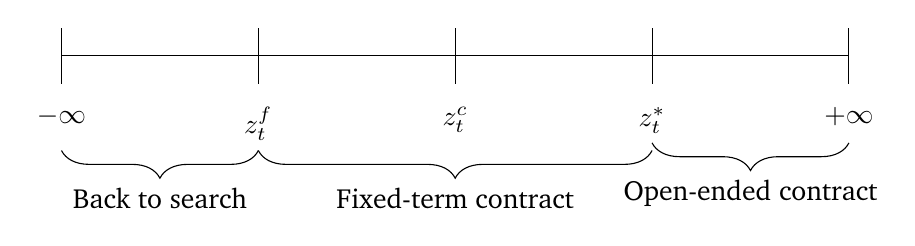
\begin{tikzpicture}[]
%draw horizontal line
\draw (0,0) -- (10cm,0);
%draw vertical lines
\foreach \x in {0,2.5,5.,7.5,10}{
   \draw (\x cm, 10pt) -- (\x cm,-10pt);
}

%draw nodes
\draw (0,0) node[below=15pt,name = zstart] {$-\infty$};
\draw (2.5cm,0) node[below=15pt,name=  zf] { $z_t^f$};
\draw (5cm,0) node[below=15pt,name=  zc] { $z_t^c$};
\draw (7.5cm,0) node[below=15pt,name = zs] {$z_t^*$};
\draw (10cm,0) node[below=15pt,name = zend] {$+\infty$};

\draw [decoration={brace,amplitude=10pt}, decorate] (zf.south) -- (zf.south -| zstart.south) node [below = 10pt, pos=0.5] {Back to search};
\draw [decoration={brace,mirror,amplitude=10pt}, decorate] (zf.south) -- (zf.south -| zs.south) node [below = 10pt, pos=0.5] {Fixed-term contract};
\draw [decoration={brace,mirror,amplitude=10pt}, decorate] (zs.south) -- (zs.south -| zend.south) node [below = 10pt, pos=0.5] {Open-ended contract};
\end{tikzpicture}
\caption{\label{fig:dual_jc} Dual job creation}
\end{figure}
\end{itemize}
\end{proposition}
\begin{proof}
See Appendix \ref{app:proofs}
\end{proof}

Demonstrating proposition \ref{prop:jc} follows the same steps as in \citet{rion:halshs-02331887}. However, the choice between open-ended contract and a fixed-term contract does not stem from the same mechanisms. Here, the trade-off opposes flexibility and productivity. An open-ended contract delivers a full productivity but may lead to the payment of firing costs if an adverse productivity shock hits. Thus, hiring an open-ended worker is worth it if productivity is high enough to overcome the expected firing costs. A fixed-term contract delivers a lower productivity, but it is shorter and separation costs zero. The option of hiring a fixed-term contract makes agents short-sighted: it pushes up the minimum productivity to hire an open-ended contract and tightens the hiring window for open-ended contracts.  

\citet{rion:halshs-02331887} is similar to the present model with two notable exceptions. Firstly, open-ended and fixed-term workers have the same productivity. Secondly, matches face i.i.d productivity shocks, whose occurrence follows a Poisson law. A new match with a high productivity chooses a contract to last as long as possible: it would be a pity to split before any productivity shock hits and to lose the advantage of a high productivity draw. Thus, on average, an open-ended contract lasts longer than a fixed-term contract and enables to lock up highly productive matches. A new match with a lower initial productivity may not find it optimal to face the risk of paying firing costs in the doldrums to secure current gains. In worst cases, going back to search is the best option. In the middle ground, though, fixed-term contracts are relevant; they enable both production and a quick return to search for a better match.

In this paper, productivity shocks no longer hit at random according to a memory-less Poisson law, which cuts out the incentive to secure the most productive matches through open-ended contracts.  When meeting, a firm and a worker know that the current productivity draw will last one period. They do not hope a high productivity draw to last forever. Thereby, Fixed-term contracts lose their role of median solution between producing and searching for more productive matches. One contract would be systematically preferred to the other without the contractual productivity gap. Still, the assumption that fixed-term contracts are \emph{per se} less productive than open-ended ones is not far-fetched. Fixed-term positions are mainly filled by low-skilled or inexperienced workers \citep{fontaine2016cdd} and benefit less from on-the-job training \citep{doi:10.1111/1467-8543.00106,10.1162/154247604323068041,Albert2005,10.1093/esr/jcs011}. \citet{doi:10.1111/ecin.12077} estimate that fixed-term workers are 20\% less productive than open-ended workers.

The main departure with \citet{sala2009flexibility} and \citet{SJOE:SJOE1715} is the appearance of the threshold $z_t^*$. The movements in thresholds $z_t^p$, $z_t^c$, $z_t^f$ and $z_t^*$ shape the behavior of the labor market and its fluctuations. If job creation involves both fixed-term and open-ended contracts --- as will be the case in my calibration --- then Figure \ref{fig:pdf} sums up the hiring and firing policies and the position of the thresholds if idiosyncratic productivity shocks are drawn from a log-Normal distribution.

\begin{figure}[H]
\begin{center}
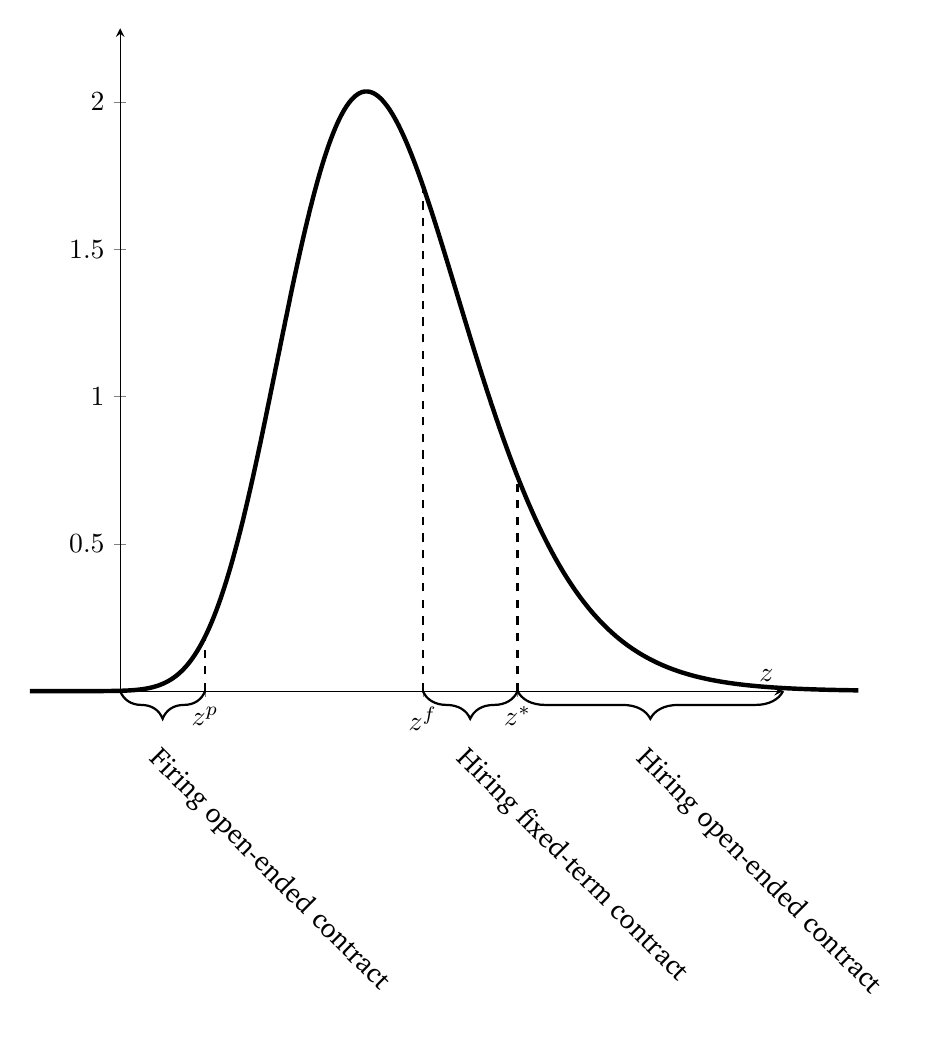
\begin{tikzpicture}

\newcommand\zp{0.62}
\newcommand\zf{1.08}
\newcommand\zs{1.28}
\newcommand\sigz{0.2}

\begin{axis}[
clip=false,
height = 10cm,
width = 10cm,
xlabel = $z$,
ylabel = {},	
xmin = exp(\sigz^2)-3*\sigz,
xmax = exp(\sigz^2)+4*\sigz,
ymin = 0.,
ymax = 2.25,
axis lines = middle,
legend pos= outer north east,
xtick = {\zp,\zf,\zs},
xticklabels={$z^p$,$z^f$,$z^*$}
]

\addplot[color = black,ultra thick,samples=1000,domain = 0.25:2.] { exp(-0.5*ln(x)^2/(0.2^2)) / (x*0.2*sqrt(2*pi))} ;
\addplot [color = black,thick,dashed]  coordinates { (\zp,0.) (\zp,{exp(-0.5*ln(\zp)^2/(0.2^2)) / (\zp*0.2*sqrt(2*pi))} ) };
\addplot [color = black,thick,dashed]  coordinates { (\zf,0.) (\zf,{exp(-0.5*ln(\zf)^2/(0.2^2)) / (\zf*0.2*sqrt(2*pi))} ) };
\addplot [color = black,thick,dashed]  coordinates { (\zs,0.) (\zs,{exp(-0.5*ln(\zs)^2/(0.2^2)) / (\zs*0.2*sqrt(2*pi))} ) };
\draw [thick,decoration={brace,mirror,amplitude = 10pt},decorate] (axis cs:{exp(\sigz^2)-3*\sigz},0.) -- (axis cs:\zp,0.) node[midway, anchor=north west, yshift=-0.5cm, rotate = -45] {Firing open-ended contract};
\draw [thick,decoration={brace,mirror,amplitude = 10pt},decorate] (axis cs:\zf,0.) -- (axis cs:\zs,0.) node[midway, anchor=north west, yshift=-0.5cm, rotate = -45] {Hiring fixed-term contract};
\draw [thick,decoration={brace,mirror,amplitude = 10pt},decorate] (axis cs:\zs,0.) -- (axis cs:{exp(\sigz^2)+4*\sigz},0.) node[midway, anchor=north west, yshift=-0.5cm, rotate = -45] {Hiring open-ended contract};
\end{axis}
\end{tikzpicture}
\end{center}
\caption{The probability distribution function of idiosyncratic shocks and the location of thresholds}
\begin{flushleft}
\small The displayed pdf belongs to a log-Normal low with zero mean and standard deviation 0.2. \normalsize
\end{flushleft}
\label{fig:pdf}
\end{figure}

\subsection{Fiscal and monetary policy}

The government taxes households in order to provide for the unemployment benefits. The revenues from the firing tax get back to the government. Thus, the budget constraint of the government is

\begin{equation}
\tau_t + (1-s) G\left( z_t^p \right) n_t^p F_t = \rho^b \overline{w_t} u_t + g_t
\end{equation}

where $g_t$ is the government expenditure and follows the AR(1) log-process $log\left(g_t\right) = \left(1-\rho_g\right) log\left(\overline{g}\right) + \rho_g log\left( g_{t-1} \right) + \epsilon_t^g$, $\epsilon_t^g \sim \mathcal{N} \left( 0, \sigma_g^2 \right)$.

The monetary policy is decided in accordance with the Taylor rule

\begin{equation}
log\left( R_{t} / R \right) = \rho_R log\left( R_{t-1} / R\right) + \left( 1 - \rho_R \right) \left[ \rho_{\pi} \mathbb{E}_t log \left( \frac{P_{t+1}}{P_t} \right) + \rho_y log\left(\frac{y_t}{y}\right) \right] + \epsilon_t^m \label{eq:taylor}
\end{equation}

where $y$ is the steady-state output and $\epsilon_t^m \overset{iid}{\sim} \mathcal{N} \left( 0, \sigma_m^2 \right)$.

Fixed-term contracts are known to behave as buffers in front of workload fluctuations, as \citet{saint1996dual} documented. Thus, the case of indeterminacy in the Taylor rule and the subsequent appearance of sunspot equilibria may prove interesting. For the sake of simplicity, though, I shall restrain the present analysis to the determinate case with $\rho_{\pi} > 1$ and $\rho_y > 0$ and leave indeterminacy and its consequences on dual labor markets for future research.

\subsection{Aggregate values and the equilibrium}

This paragraph sums up the different conditions enabling an utter closing of the model. The employment values sum to the measure of households, namely 1.

\begin{equation}
n_t^p + n_t^f + u_t = 1
\end{equation}

$n_t^p$, $n_t^f$ and $u_t$ are the measures of open-ended employees, fixed-term employees and unemployed workers.

The aggregate stock of job-seekers includes the formerly unemployed households and the new entrants in the unemployment pool from the current period.

\begin{equation}
e_t = u_{t-1} + \delta n_{t-1}^f + \xi_t n_{t-1}^p
\end{equation}

The labor market tightness is the ratio between aggregate number of vacancies $v_t = \int_{0}^{1} v_{i,t} di$ and the number of job seekers.

\begin{equation*}
\theta_t = \frac{v_t}{e_t}
\end{equation*}

The employment variables drop by the job destruction flow and augment by the job creation flow.

\begin{align}
n_t^p &= \left( 1 - \xi_t \right) n_{t-1}^p + \mu_t^p e_t\\
n_t^f &= \left( 1 - \delta \right) n_{t-1}^f + \mu_t^f e_t
\end{align}

where $\mu_t^p = p\left( \theta_t \right) \left( 1- G\left( z_t^*\right)\right)$ and $\mu_t^f = p\left( \theta_t \right) \left( G\left( z_t^*\right)-G\left( z_t^f \right)\right)$ are the open-ended and fixed-term job-finding rates. $\xi_t = s + (1-s) G\left( z_t^p \right)$ is the the job destruction rate of open-ended contracts.

As for firms, the aggregate demand for final goods is

\begin{equation}
Y_t = c_t + g_t + \gamma v_t \label{eq:res_cons}
\end{equation}

The retailers face only one real marginal cost from the intermediate firms, which entails a unique equilibrium value for the optimal price-setting program, \emph{id est} $P_{i,t}^* = P_t^*$.

The market clearing condition for intermediate goods states that intermediate goods are produced by incumbent workers or new workers through either open-ended or fixed-term contracts. 

\begin{align*}
\int_{0}^{1} Y_{i,t} di &= A_t E_z \left[z \mid z \geq z_t^p \right] \left( 1 - \xi_t \right) n_{t-1}^p + \left( 1 - G\left( z_t^* \right)\right) q \left( \theta_t \right) v_t A_t E_z \left[z \mid z \geq z_t^* \right]\\
&+ \rho A_t \mathbb{E}_z \left[ z \right] \left( 1 - \delta \right) n_{t-1}^f + \rho \left( G\left( z_t^* \right) - G\left( z_t^f \right)\right) q \left( \theta_t \right) v_t A_t \mathbb{E}_z \left[z \mid z_t^* \geq z \geq z_t^f \right]
\end{align*}

Using the first order condition from the final good firm's program \eqref{eq:ret_dem}, I get

\begin{align}
\begin{split}
Y_t \Delta_t &= A_t E_z \left[z \mid z \geq z_t^p \right] \left( 1 - \xi_t \right) n_{t-1}^p + \left( 1 - G\left( z_t^* \right)\right) q \left( \theta_t \right) v_t A_t E_z \left[z \mid z \geq z_t^* \right]\\
&+ \rho A_t E_z \left[ z \right] \left( 1 - \delta \right) n_{t-1}^f + \rho \left( G\left( z_t^* \right) - G\left( z_t^f \right)\right) q \left( \theta_t \right) v_t A_t E_z \left[z \mid z_t^* \geq z \geq z_t^f \right] \label{eq:res_cons_int}
\end{split}
\end{align}

with $\Delta_t = \int_{0}^{1} \left( \frac{P_{i,t}}{P_t}\right)^{-\epsilon_t} di$ which measures price dispersion. \citet{yun1996nominal} demonstrated that the associated law of motion is

\begin{equation}
\Delta_t = (1-\psi) \left( \frac{P_t^*}{P_t} \right)^{-\epsilon_t} + \psi \left( \frac{P_t}{P_{t-1}} \right)^{\epsilon_t} \Delta_{t-1}
\end{equation}

while the price level follows

\begin{equation}
P_t = \left[ \psi P_{t-1}^{1-\epsilon_t} + (1-\psi) \left( P_t^* \right)^{1-\epsilon_t} \right]^{\frac{1}{1-\epsilon_t}} \label{eq:lm_price}
\end{equation}

Average wages pinpoint unemployment benefits as well as firing costs. Firing costs are a share of the average wage of incumbent open-ended workers. Denoting $\widetilde{w_t^p}$ the average wage of incumbent workers with open-ended contracts, firing costs verify

\begin{align}
F_t = \rho^F \widetilde{w_t^p}
\end{align}

The average wage of incumbent open-ended workers is simply the expected wage of open-ended matches with a productivity higher than the firing threshold.

\begin{align*}
\widetilde{w_t^p} &= \mathbb{E}_t \left[ w_t^p \left( z \right) \mid z \geq z_t^p\right]
\end{align*}

Using \eqref{eq:wp}, the average wage of incumbent open-ended workers boils down to

\begin{align}
\widetilde{w_t^p} &= \eta \left( A_t \phi_t \mathbb{E}_t \left[ z \mid z_t^p \leq z \right] + F_t - E_t \beta_{t,t+1} (1-s) F_{t+1} + \gamma \theta_{t} \right) + (1-\eta) b_t
\end{align}

The average wage of open-ended workers includes the wage that are not fired and with productivity higher than the firing threshold.

\begin{align*}
\overline{w_t^p} &= \frac{\left( 1-\xi_t \right) n_{t-1}^p \mathbb{E}_t \left[ w_t^p \left( z \right) \mid z \geq z_t^p\right] + \mu_t^p e_t \mathbb{E}_t \left[ w_t^{0,p} \left( z \right) \mid z \geq z_t^*\right]}{n_t^p}\\
\overline{w_t^f} &= \frac{\left( 1-\delta \right) n_{t-1}^f\mathbb{E}_t \left[ w_t^f \left( z \right) \right] + \mu_t^f e_t \mathbb{E}_t \left[ w_t^{f} \left( z \right) \mid z_t^f \leq z \leq z_t^*\right]}{n_t^f}\\
\end{align*}

Given the path of exogenous shocks $\left\{ \epsilon_t^A, \epsilon_t^\mu, \epsilon_t^g, \epsilon_t^m \right\}_{t=0}^{+\infty}$, laws of motions of exogenous shocks $\left\{ A_t, \mu_t , g_t \right\}_{t=0}^{+\infty}$ and initial values for the state variables $\left\{ R_{-1}, n_{-1}^p, n_{-1}^f, \Delta_{-1}, P_{-1} \right\}$, the equilibrium sums up into the set of endogenous variables $\left\{ R_t, c_t, Y_t, n_t^p, n_t^f, u_t, \Delta_t, z_t^p, z_t^c, z_t^f, z_t^*, \theta_t, \phi_t, v_t, P_t, P_t^*, b_t, F_t, \overline{w_t^p}, \overline{w_t^f}, \widetilde{w_t^p} \right\}_{t=0}^{+\infty}$ pinned down by equations \eqref{eq:euler_eq}, \eqref{eq:price_eq}, \eqref{eq:zp}-\eqref{eq:zf}, \eqref{eq:zs} and \eqref{eq:taylor}-\eqref{eq:lm_price}. 
\input{calibration}
%
\section{Experiments}

\subsection{Labor market moments}

\begin{figure}[t]
\begin{center}
\includegraphics[scale=1.]{lm_moments.pdf}
\caption{Fluctuations in labor market values.}
\label{fluctuations}
\end{center}
\end{figure}

In this paragraph, we assess the ability of the model with respect to the reproduction of labor market moments. The absence of proper series for the computation of the latter in the Euro area represents a significant obstacle. As a result, I use series draws from French data as a proxy to account for the main features of a dual labor market.

The series are logged and filtered along the lines of \citet{hamilton2018you}. Importantly, I do not use the so-called Hodrick-Prescott filter, whether it be one-sided or two-sided. Indeed, \citet{hamilton2018you} explains the purely artifical statistical properties of series filtered through the Hodrick-Prescott method. The use of the Hodrick-Prescott filter imposes strong statistical properties on series because of its inner structure, regardless the process behind the actual data. Stunningly, when considering random walks, the output of the Hodrick-Prescott filter presents persistence. This behavior of the Hodrick-Prescott filter is all the more worrying since macroeconomic time series often boil down to martingales, whose increments remain unpredictable by definition. In standard macroeconomic samples of data, a band pass filter only captures the frequencies belonging to cycles with periodicity between 5 and 40 quarters. Considering growth rates exaggerates the high frequency margin in the data. Overall, a filtering method remains an arbitrary choice with many pitfalls\footnote{See \citet{gorodnichenko2010estimation}, \citet{ferroni2011trend}, \citet{lafourcade2012taking}, \citet{canova2014bridging} and \citet{hamilton2018you} for thorough developments of this idea}.

\begin{table}[H]
\begin{center}
\begin{tabular}{ccccc}
\toprule
 Variables & \multicolumn{2}{c}{Data} & \multicolumn{2}{c}{Model} \\ \cmidrule(lr){2-3} \cmidrule(lr){4-5} & Std. Dev. & $Cor\left( Y, . \right)$ & Std. Dev. & $Cor\left( Y, . \right)$ \\ \midrule 
$Y$ & 1.16 & 1.0 & 0.9 & 1.0 \\ 
$\pi$ & 0.32 & 0.15 & 0.32 & -0.02 \\ 
$R$ & 0.33 & 0.29 & 0.21 & 0.31 \\ 
$n$ & 0.73 & 0.93 & 1.0 & 0.86 \\ 
$jc^p$ & 7.19 & 0.65 & 10.41 & 0.37 \\ 
$jc^f$ & 4.97 & 0.52 & 5.63 & 0.08 \\ 
$\mu^f / \left( \mu^f + \mu^p \right)$ & 1.29 & -0.4 & 2.71 & -0.35 \\ 
$n^f$ & 1.87 & 0.18 & 2.67 & 0.06 \\ 
$jd^p$ & 5.26 & -0.46 & 17.84 & -0.47 \\ 
$jd^f$ & 2.84 & 0.39 & 2.66 & -0.05 \\ 
$v$ & 10.32 & 0.61 & 6.08 & 0.24 \\ 
\bottomrule
\end{tabular}
\caption{Actual and simulated correlations with output of different variables}
\end{center}
\begin{flushleft}
\footnotesize{For each of the 10,000 particles from the SMC algorithm, the correlations are computed over 400-period chains of shocks after a 100-period burn-in time. A weighted average of these moments is then derived using the particle-specific weights generated by the SMC procedure.}
\end{flushleft}
\end{table}

\subsection{Impulse Response Functions}

The computation of impulse response functions highlights several interesting features of the model. First of all, a substitution effect between temporary and permanent contracts emerges, with long-run consequences on employment whether it be temporary or permanent and a strong influence on impact. Secondly, a general-equilibrium effect appears. Indeed, shocks imply changes in the size of the job seekers' pool, which, in turn, has important implication for job creation flows. Finally, the common source of both effects being the evolution of $\left( z^p, z^f, z^*, \theta\right)$, the two effects interact through time depending on the persistence of the considered shock.

\begin{figure}[t]
\includegraphics[scale=1]{irf_A.pdf}
\caption{IRF of main variables to a one-standard-deviation productivity shock}
\label{IRF_A}
\end{figure}

\paragraph{Productivity shocks} Figure \ref{IRF_A} displays the reaction of main variables to a productivity shock. An increase in labor productivity cuts real marginal costs. Inflation decreases and the central bank reduces nominal interest rates to encourage consumption. The support to demand is insufficient to prevent a decrease in employment. Unemployment increases while vacancies reduce, delineating a downward-sloping Beveridge curve and a decrease in labor market tightness. These results are classic in DSGE models with nominal rigidities. The downward sloping Beveridge curve is a traditional feature of Mortensen Pissarides models.

The behavior of flows constitute an important feature of labor markets. The enhanced productivity fuels higher job destruction among permanent contracts ; $z^p$ increases. Firms are more reluctant to keep low-productivity permanent matches as their expected gain from searching a worker enlarges. Job creation, as for it, immediately decreases through both permanent and temporary contracts because of of the drop in labor demand. Interestingly, job creation ends up increasing a few quarters after the observed cut on impact. This comes from a general equilibrium effect. Just after the shock, aggregate job destruction increases and job creation shrinks, which inflates the job seekers' pool for the next periods. This mechanically increases the subsequent job creation flows. On impact, output decreases because of the shrink in employment, which overcomes the productivity gains. Thereafter, the recovery of job creation pushes it up. 

The movements in thresholds $z^f$ and $z^*$ are key. The enhanced productivity makes firms' hiring policy more stringent and worker-firm pairs are more exacting about the productivity of an accepted match when they meet ; $z^f$ enlarges. The forces at stake when it comes to the evolution of $z^*$ are more complex. On one hand, the agents seek to benefit from productivity gains in full, which bolsters the attractiveness of permanent workers. On the other hand, firms are more demanding in terms of productivity when hiring a new permanent worker. On impact, the latter effect prevails, but it is quickly overcome by the former. The choice between a temporary and a permanent contract at the hiring stage also reflects the compromise between the fear of future rigidity and the appetite for productivity gains. Overall, productivity gains are insufficient to encourage substitution in favor of permanent contracts ; the transitory nature of the shock encourages the resort to temporary contracts, and the share of temporary contracts in job creation increases\footnote{This behavior stems from the location $z^f$ and $z^*$ occupy on the support of the distribution of idiosyncratic shocks, which Figure \ref{fig:pdf} shows. Movements in $z^f$ concern more formerly viable matches than similar movements in $z^*$, the slope of the probability density function of idiosyncratic shocks being higher in the neighborhood of $z^f$.}. Permanent employment unambiguously shrinks under the joint diminution in job creation and increase in job destruction. As for temporary contracts, job creation shrinks and job destruction occurs at a constant exogenous rate. Consequently, temporary employment decreases. 

\begin{figure}[t]
\includegraphics[scale=1]{irf_g.pdf}
\caption{IRF of main variables to a one-standard-deviation shock in government spending shock}
\label{IRF_g}
\end{figure}

\paragraph{Government spending shocks} Figure \ref{IRF_g} shows the impulse response functions of main variables after a shock in government spending. As usual in the literature, a sudden increase in government spending enhances output. Real marginal costs increase and the central bank increases the nominal interest rate to prevent the spread of inflation. The labor market tightness increases as firms post more vacancies to cope with the magnified demand of consumption goods. As a result, on impact, job destruction decreases and job creation increases. Interestingly, firms cope with the surplus of demand through an enlarged share of permanent contracts in job creation. The shock is persistent enough for the future expected losses associated with firing costs to be overcome by lifelong productivity gains. The general-equilibrium effect described in the preceding sections weighs in anew. Indeed, the shrink in the job seekers' stock exerts a downward pressure on job creations, which decrease below their steady-state values. While the transitional path of permanent employment remains above its steady-state value, temporary employment goes below its equilibrium level. As a matter of fact, fixed-term employment experiments a higher turnover, and is therefore highly impacted by temporary fluctuations in its associated job creation\footnote{This is all the more true since destruction rates of temporary jobs are constant}.

\begin{figure}[t]
\includegraphics[scale=1]{irf_m.pdf}
\caption{IRF of main variables to a one-standard-deviation in the monetary policy shock}
\label{IRF_m}
\end{figure}

\paragraph{Monetary policy shock} Figure \ref{IRF_m} shows the impulse response functions of main variables after a shock in the monetary policy. A monetary policy shock pushes up interest rates, which discourages consumption and subsequently depresses output. Real marginal costs and inflation decrease. The marginal gross revenue from labor decreases and intermediate firms are overall more demanding in productivity terms to compensate the loss in profits ; firms post fewer vacancies and $z^p$ as well as $z^f$ increase. Thus, on impact, the labor market tightness shrinks and permanent job destruction enlarges. In turn, the formerly permanent employees join the ranks of the job seekers', which enhances job creation. Moreover, firms tend to switch to permanent contracts on behalf of temporary ones at the hiring stage in order to temper the immediate loss in revenue due to prices ; $z^*$ decreases. These two effects combined explain the observed rebound in permanent job creation.

As a result, viewed from the labor market, the monetary policy shock represents the negative of the government spending shock. The economic schemes at stake are the same. There is however a nuance. The effects of the monetary policy shock on the interest rate vanish much faster and the oscillations between the substitution effect and the general-equilibrium effect develop in a rougher way. This observation is also relevant when one considers the cost-push shock. The IRF of the latter will not be described, as it involves the same economic phenomena as the other shocks.

\subsection{Reforms in employment protection legislation}

In this paragraph, I examine the macroeconomic effects of a reform on employment protection legislation, which is summed up in firing costs here. I consider both transitory and permanent shocks. Transitory shocks are interesting, as employment protection legislation has frequently been the target of many reforms in Europe. \citet{fontaine2016cdd}, quoting a report from an observatory of the European Commission, mention the implementation of more than 220 policies related to employment protection legislation between 2005 and 2013. Permanent shocks, as for them, are relevant to study changes in volatilities of inflation, employment or output for example.

\begin{figure}[t]
\includegraphics[scale=1]{irf_F.pdf}
\caption{IRF of main variables after a one-per-cent shock in firing costs}
\label{IRF_F}
\end{figure}

Figure \ref{IRF_F} displays the reaction of main variables to a one-percent positive shock to firing costs. The process for the logged shock is supposed to be an AR(1) with auto-regressive coefficient 0.8, so that the shock vanishes at 99\% five years after the impact. An increase in firing costs discourages job destruction ; $z^p$ and $jd^p$ decrease. Two opposite effects weigh on the composition of job creation. On one hand, enlarged firing costs entail costlier endogenous separations, which encourages substitution towards temporary job creation. On the other hand, these endogenous separations are scarcer. As a result, firms are less demanding in terms of productivity when it comes to hiring a permanent worker, which favors substitution towards permanent employment. In the present case, the former effect prevails ;  the share of temporary contracts in job creation increases.

Interestingly, the expected gain from posting a vacancy decreases because of the shrinking share of open-ended contracts in job creations. The resulting decrease in vacancy-filling rate joint with the tightened threshold for permanent hires reduces permanent job creation expands. The reduction in the permanent job destruction rate does no overcome the depleted permanent job creation rate and permanent employment dwindles. The substitution effect towards temporary contracts increases temporary job creation and temporary employment, as temporary job destruction occurs at a constant rate. Overall, output decreases. Inflation persistently increases in a hump-shaped manner even though the size of the response is small. Interestingly, a marginal and temporary change in firing costs generates long-lasting effects on inflation.

\begin{figure}[t]
\includegraphics[scale=1]{NKPC.pdf}
\caption{The weight of permanent contracts in inflation dynamics in function of steady-state firing costs.}
\label{NKPC}
\footnotesize
\begin{flushleft}
The x-axis represents the percentage deviation of steady-state firing costs with respect to the baseline calibration, which is set at 0.
\end{flushleft}
\end{figure}


In order to understand the dynamics of inflation, I derive the New-Keynesian Phillips curve associated with the present model as is classic in the literature and find

\begin{align*}
\widehat{\pi_t} = \beta \mathbb{E}_t \widehat{\pi_{t+1}} + \kappa \left( \widehat{\mu_t} + \widehat{\phi_t} \right)
\end{align*}

where $\kappa = (1-\beta \psi) (1-\psi) / \psi$.

Meanwhile, I use the job creation condition to isolate $\phi_t$ and obtain

\begin{align*}
\phi_t = \frac{\gamma}{ (1-\eta) A_t \left[ \left( E_z \left[ z \middle| z \geq z_t^* \right] - z_t^c \right) q\left( \theta \right) \left( 1 - G\left( z_t^* \right)\right) + \rho \left( E_z \left[ z \middle| z_t^f \leq z \leq z_t^* \right] - z_t^f \right) q\left( \theta \right) \left( G\left( z_t^* \right) - G\left( z_t^f \right)\right) \right] }
\end{align*}  

The left-hand-side term in the bracketted part of the denominator is the expected surplus of production from a hire through permanent contract $\psi_t^p$ weighted with its probability of occurence $\mu_t^p$. This so-called surplus of production is the production of the match beyond the one corresponding to the zero-profit point. In an analogous manner, the right-hand-side term is the expected surplus of production from a hire through a temporary contract $\psi_t^f$ weighted by its probability of occurence $\mu_t^f$. Overall, the real marginal cost evolves negatively with the ability of the labor market to generate in expectations such production surpluses. This reminds the simple rule of a decreasing cost with respect to the abundance of a given good. Log-linearizing this condition and assuming that there are neither cost-push shocks nor productivity shocks, the New-Keynesian Phillips curve becomes

\begin{align*}
\widehat{\pi_t} = \beta \mathbb{E}_t \widehat{\pi_{t+1}} - \kappa \frac{\mu^p \psi^p}{\mu^p \psi^p + \mu^f \psi^f} \left( \widehat{\mu_t^p} + \widehat{\psi_t^p} \right) - \kappa \frac{\mu^f \psi^f}{\mu^p \psi^p + \mu^f \psi^f} \left( \widehat{\mu_t^f} + \widehat{\psi_t^f} \right)
\end{align*}

Retailers benefit from their market power and extract a rent from the production that exceeds intermediate firms' profitability thresholds. Interestingly, the discounted innovation in inflation is a weighted average, with the steady-state share of the newly hired workers' production for each contract as weights. The magnitude of these weights is difficult to assess, to the extent that they reflect a trade-off between a high hiring probability and a low average productivity, and conversely. The determinants of inflation dynamics are directly related to the evolution of the contractual composition of hires and their productivity. Figure \ref{NKPC} shows the importance of fluctuations on the permanent side of the labor market with different values of $F$, 0 being the baseline calibration. When $F$ increases, the weight of permanent contracts in the shaping of inflation dynamics decreases. As permanent job destruction becomes scarcer, the agents are less exacting in the productivity of hired permanent workers, which overcomes the enhanced permanent job creation ; the permanent side of the labor market loses importance when considering inflation dynamics. Importantly, these results highly depend on the distribution of idiosyncratic shocks. Nevertheless, as we changed $\sigma_z$ to 0.1 or 0.15, there were no notable difference in the results\footnote{An interval of values for the standard deviation of distribution of idiosyncratic productivity shocks $\sigma_z$ over which steady-state quantities are plausible is $( 0.1 , 0.22 )$}. Another important factor that influences inflation dynamics is the adjustment speed of employments, which is small in a labor market where flows are constrained by employment protection legislation. Consequently, reforms in employment protection legislation generate significant and persistent fluctuations in inflation. The size of the subsequent perturbations is small, though. A 10-per-cent cut in firing costs typically entails a 30-basis-point decrease in inflation on impact.
%\section{Conclusion}

In this paper, I show the importance of the contractual composition with respect to labor market flows when it comes to understand fluctuations on a dual labor market. The estimated model replicates well the main moments of a typical European dual labor market. Our approach highlights the importance of a contractual substitution effect at the hiring stage and the general-equilibrium effect it fuels by impacting the job seekers' pool. Inflation dynamics reflect the firms' hiring choices in contractual terms. As a result, employment protection legislation reforms directly impact inflation dynamics.

A few points merit further discussion, though. A potential issue in the current analysis is the implicit assumption that the labor market \emph{is} at the steady state. According to the data, temporary employment in the Euro area seems to have stabilized since the beginning of the 2000s, but the exponential rise of temporary employment between the 80s and 2000 may cast doubt on its future behavior. The absence of endogenous quitting decisions is also a limitation that needs to be highlighted, especially in the Euro Area where voluntary job-to-job transition represent a substantial share of permanent job separations and probably present a sharp pro-cyclical behavior. The exogenous character of the productivity distribution and its independence of other shocks also constitutes a problem, because this makes the model sensitive to the Lucas critique. Indeed, an employment protection legislation reform probably may modify firms' productivity distributions. With these critiques in mind, my findings should be considered as an incentive to consider the contractual composition of labor market flows in an endogenous manner when short-term horizons and monetary policy are considered.


%\newpage

%\bibliographystyle{elsarticle-harv}
%\bibliography{ch2}

\newpage

\appendix

\section{Detailed Calculations}

\subsection{Nash-bargaining joint surpluses}
\label{sec:nb_surplus}

Using the different definitions of surpluses with the free-entry condition -namely equations \eqref{eq:def_jp}, \eqref{eq:def_wp}, \eqref{eq:free_entry} and \eqref{eq:def_sp} - I get

\begin{align} \label{eq:sp_appendix}
\begin{split}
S_t^p \left( z_t \right) &= z_t - U_t + F_t - \mathbb{E}_t \beta_{t,t+1} (1-s) F_{t+1}\\
&+ \mathbb{E}_t  \beta_{t,t+1} \left\{ (1-s)\int_{z_{t+1}^p}^{+\infty} S_{t+1}^p (z) dG(z) + \left(1-\xi_{t+1}\right) U_{t+1} + \xi_{t+1} \widehat{U_{t+1}}\right\}
\end{split}
\end{align}

Meanwhile, the definition of $\widehat{U_t}$ \eqref{eq:def_uhat} yields

\begin{align}
\widehat{U_t} = U_t + p\left(\theta_t \right) \left( \int_{H_t^p} \left( W_t^{0,p} (z) - U_t \right) dG(z) + \int_{H_t^f} \left( W_t^{f} (z) - U_t \right) dG(z) \right)
\end{align}

Nash-sharing rules \eqref{eq:nash_0p} imply that
\begin{align}
\widehat{U_t} = U_t + \frac{\eta}{1-\eta} p\left(\theta_t \right) \left( \int_{H_t^p} J_t^{0,p} (z) dG(z) + \int_{H_t^f} J_t^f (z) dG(z) \right)
\end{align}

But \eqref{eq:def_v} and \eqref{eq:free_entry} imply that
\begin{align}
\int_{H_t^p} J_t^{0,p} (z) dG(z) + \int_{H_t^f} J_t^f (z) dG(z) = \frac{\gamma}{q\left( \theta_t \right)}
\end{align}

Since $p \left( \theta_t \right) = \theta_t q \left( \theta_t \right)$, the definition of $\widehat{U_t}$ boils down to

\begin{align}
\widehat{U_t} = U_t + \frac{\eta \gamma \theta_t}{1-\eta} \label{eq:nash_uhat}
\end{align}

Consequently, the present discounted value of unemployment equals

\begin{align}
U_t = b + \mathbb{E}_t \beta_{t,t+1} U_{t+1} + \mathbb{E}_t \beta_{t,t+1} \frac{\eta \gamma \theta_{t+1}}{1-\eta} \label{eq:nash_u}
\end{align}

Reintroducing \eqref{eq:nash_uhat} and \eqref{eq:nash_u} into \eqref{eq:sp} leads to the following expression for the surplus of continuing permanent contracts

\begin{align}
\begin{split}
S_t^p \left( z_t \right) &= A_t z_t \phi_t - b + F_t - \mathbb{E}_t \beta_{t,t+1} (1-s) F_{t+1} - \mathbb{E}_t \beta_{t,t+1} \left( 1 - \xi_{t+1} \right) \frac{\eta \gamma \theta_{t+1}}{1-\eta}\\
&+ \mathbb{E}_t  \beta_{t,t+1} (1-s) \int_{z_{t+1}^p}^{+\infty} S_{t+1}^p (z) dG(z)
\end{split}
\end{align}

Following the same steps, I find that

\begin{align}
S_t^{0,p} \left( z_t \right) = S_t^p \left( z_t \right) - F_t
\end{align}


As for temporary contracts, equations \eqref{eq:def_jf}, \eqref{eq:def_wf} and \eqref{eq:free_entry} boil down to

\begin{align}
S_t^f \left( z_t \right) = \rho A_t z_t \phi_t - U_t + \mathbb{E}_t \beta_{t,t+1} \left\{ (1-\delta) \int S_{t+1}^f (z) dG(z) + (1-\delta) U_{t+1} + \delta \widehat{U_{t+1}} \right\}
\end{align} 

Using \eqref{eq:nash_uhat} and \eqref{eq:nash_u}, the surplus of temporary contracts is

\begin{align}
S_t^f \left( z_t \right) = \rho A_t z_t \phi_t - b - \mathbb{E}_t \beta_{t,t+1} (1-\delta) \frac{\eta \gamma \theta_{t+1}}{1-\eta} + \mathbb{E}_t \beta_{t,t+1} (1-\delta) \left\{  \int S_{t+1}^f (z) dG(z) \right\} 
\end{align}

Notice that $\partial S_t^p / \partial z_t = A_t \phi_t$ and $\partial S_t^f / \partial z_t = \rho A_t \phi_t$ Moreover, $S_t^p \left( z_t^p \right) = 0$ and $S_t^f \left( z_t^f \right) = 0$ by definition. Thus, integration by parts lead to the following expressions for continuing permanent matches and temporary matches

\begin{align}
\begin{split}
S_t^p \left( z_t \right) &= A_t z_t \phi_t - b + F_t - \mathbb{E}_t \beta_{t,t+1} (1-s) F_{t+1} - \mathbb{E}_t \beta_{t,t+1} \left( 1 - \xi_{t+1} \right) \frac{\eta \gamma \theta_{t+1}}{1-\eta}\\
&+ \mathbb{E}_t  \beta_{t,t+1} (1-s) A_{t+1} \phi_{t+1} \int_{z_{t+1}^p}^{+\infty} \left( 1 -  G(z) \right) dG(z)
\end{split}\\
S_t^f \left( z_t \right) &= \rho A_t z_t \phi_t - b - \mathbb{E}_t \beta_{t,t+1} (1-\delta) \frac{\eta \gamma \theta_{t+1}}{1-\eta} + \rho \mathbb{E}_t \beta_{t,t+1} (1-\delta) A_{t+1} \phi_{t+1} \left( \mathbb{E}z - z_{t+1}^f \right) 
\end{align}

\subsection{Steady-state equations}

Given the parameters $\beta, \sigma, \eta, \sigma_z, \epsilon, F, b, , \delta, \rho, m, \gamma$, we need to derive the steady-state values of the variables $R, c, Y, n^p, n^f, u, \Delta, z^p, z^c, z^f, z^*, \theta, \phi, v, \pi,  A, \mu , g$. Some of them can be directly computed through the following equations

\begin{align*}
R &= 1/\beta \\
\mu &= 1/\phi\\
\phi &= \frac{\epsilon - 1}{\epsilon}\\
P &= P^* = \Delta = 1\\
A &= 1
\end{align*}

Given $\left( z^p , \theta \right)$, $\left( q, \xi, z^f, z^c, z^* \right)$ can be directly derived.

\begin{align*}
q &= m \theta^{-\sigma}\\
\xi &= s+(1-s)G\left( z^p \right)\\
z^c &= z^p + \frac{F}{\phi}\\
z^f &= \frac{b + \beta (1-\delta) \left( \frac{\eta \gamma \theta}{1-\eta} - \rho \phi \mathbb{E}z \right)}{\rho \phi (1-\beta (1-\delta))}\\
z^* &= \frac{z^c - \rho z^f}{1-\rho}
\end{align*}

It is then possible to solve the following system in $\left( z^p , \theta \right)$.

\begin{align*}
&\phi z^p + \left[ 1 - (1-s)  \beta \right] F + (1-s)  \beta \phi \int_{z^p}^{+\infty} \left( 1 - G(z) \right) dz = b + \beta \left( 1 - \xi \right) \frac{\eta \gamma \theta}{1-\eta}\\
&\frac{\gamma}{(1-\eta) \phi q\left( \theta \right)} = \int_{z^*}^{+\infty} \left[ 1 - G(z) \right] dz + \rho \int_{z^f}^{z^*} \left[ 1 - G(z) \right] dz\\
\end{align*}

At this point, the values $\left( z^p , \theta, q, \xi, z^f, z^c, z^* \right)$ are known. One can compute right away $p$, $\mu^p$ and $\mu^f$.

\begin{align*}
p &= \theta q\\
\mu^p &= p \left( 1-G\left( z^*\right)\right)\\
\mu^f &= p \left( G\left( z^*\right) - G\left( z^f\right)\right)
\end{align*} 

Pinpointing $\left( n^p, n^f, u, e\right)$ involves the following linear system.

\begin{align*}
    &n^p + n^f + u = 1\\
    &e = u + \delta n^f + \xi n^p\\
    &n^p =  \left(1-\xi\right) n^p + \mu^p e\\
    &n^f =  \left(1-\delta\right) n^f + \mu^f e
\end{align*}

Solving this system yields

\begin{align*}
n^p &= \frac{\delta \mu^p}{\xi (1-\delta) \mu^f + \delta (1-\xi) \mu^p + \xi \delta}\\
n^f &= \frac{\xi \mu^f}{\xi (1-\delta) \mu^f + \delta (1-\xi) \mu^p + \xi \delta}\\
u &= 1-n^p-n^f\\
e &= u+\xi n^p + \delta n^f
\end{align*}

Now, the steady-state values $v$, $Y$, $g$ and $c$ can be obtained.

\begin{align*}
v &= \theta e\\
\begin{split}
Y &= \left(1-\xi\right) \mathbb{E}_z \left[z \mid z \geq z^p \right] n^p + \mu^p \mathbb{E}_z \left[z \mid z \geq z^* \right] e\\
&+ \rho \left(1-\delta\right)  \mathbb{E}_z \left[ z \right]  n^f + \rho \mu^f \mathbb{E}_z \left[z \mid z^* \geq z \geq z^f \right] e\\
\end{split}\\
g &= Y \left( \frac{g}{Y} \right)\\
c &= Y-g-\gamma v
\end{align*}

\newpage 
\subsection{Log-linearization}

The Euler equation can be derived from \eqref{eq:euler_eq}-\eqref{eq:def_um}.

\begin{equation*}
    u' \left( c_t \right) = \beta R_t \mathbb{E}_t \left[ \frac{P_t}{P_{t+1}} u' \left( c_{t+1} \right) \right]
\end{equation*}

which becomes

\begin{equation}
    \widehat{c_t} = \widehat{E_t c_{t+1}} - \left[-\frac{c u''}{u} \right]^{-1} \left( \widehat{R_t} - \widehat{E_t \pi_{t+1}}\right)
\end{equation}

where $\pi_t = P_t / P_{t-1}$ denotes inflation.

The definition of price level dynamics \eqref{eq:lm_price} can be log-linearized as

\begin{equation}
    \widehat{\pi_t} = (1-\psi) \left( \widehat{P_t^*} - \widehat{P_{t-1}} \right) \label{eq:lm_price_ll}
\end{equation}

The retailers' price-setting equation \eqref{eq:price_eq} becomes

\begin{equation}
    \widehat{P_t^*} = (1-\beta\psi) \mathbb{E}_t \sum_{k=0}^{+\infty} (\beta\psi)^{k} \left( \widehat{P_{t+k}} + \widehat{\mu_{t+k}} + \widehat{\phi_{t+k}} \right)
\end{equation}

Substracting $\widehat{P_{t-1}}$ on each side of this equation, we get

\begin{align}
    \widehat{P_t^*} - \widehat{P_{t-1}} &= (1-\beta\psi) \mathbb{E}_t \sum_{k=0}^{+\infty} (\beta\psi)^{k} \left( \widehat{P_{t+k}} - \widehat{P_{t-1}} + \widehat{\mu_{t+k}} + \widehat{\phi_{t+k}} \right)\\
    &= \sum_{k=0}^{+\infty} (\beta\psi)^{k} \mathbb{E}_t \widehat{\pi_{t+k}} + (1-\beta\psi) \sum_{k=0}^{+\infty} (\beta\psi)^{k}  \mathbb{E}_t \left( \widehat{\mu_{t+k}} + \widehat{\phi_{t+k}} \right)\\
    &= \beta \psi \left( \mathbb{E}_t \widehat{P_{t+1}^*} - \widehat{P_{t}} \right) + (1-\beta \psi) \left( \widehat{\mu_t} + \widehat{\phi_t}\right) + \widehat{\pi_t}
\end{align}

Using \eqref{eq:lm_price_ll}, we get

\begin{align}
\widehat{\pi_t} = \beta \mathbb{E}_t \widehat{\pi_{t+1}} + \kappa \left( \widehat{\mu_t} + \widehat{\phi_t} \right)
\end{align}

where $\kappa = (1-\beta \psi) (1-\psi) / \psi$.

The log-linearization of exogenous processes yields

\begin{align*}
\widehat{A_t} &= \rho_A \widehat{A_{t-1}} + \epsilon_t^A\\
\widehat{\mu_t} &= \rho_\mu \widehat{\mu_{t-1}} + \epsilon_t^\mu\\
\widehat{g_t} &= \rho_g \widehat{g_{t-1}} + \epsilon_t^g
\end{align*}

The other log-linearizations of equations \eqref{eq:zp}-\eqref{eq:zf}, \eqref{eq:zs} and \eqref{eq:taylor}-\eqref{eq:res_cons_int} yield

\begin{align*}
\begin{split}
&A \phi z^p \left( \widehat{A_t} + \widehat{z_t^p} + \widehat{\phi_t} \right) - \left( A \phi z^p + F - b \right) \left( c_t - \mathbb{E}_t \widehat{c_{t+1}}\right)\\
&+ \beta (1-s) A \phi \int_{z^p}^{+\infty} \left( 1-G(z)\right) dz \left( \mathbb{E}_t \widehat{A_{t+1}} + \mathbb{E}_t \widehat{\phi_{t+1}} \right)\\
&-\beta (1-\xi) \frac{\eta \gamma \theta}{1-\eta} \mathbb{E}_t \theta_{t+1} + \beta (1-s) z^p \left( - A \phi \left( 1-G\left( z^p \right) \right) + \frac{\eta \gamma \theta}{1-\eta} g\left( z^p\right) \right) \mathbb{E}_t \widehat{z_{t+1}^p} = 0
\end{split}\\
\begin{split}
&\rho A \phi z^f \left( \widehat{A_t} + \widehat{z_t^f} + \widehat{\phi_t} \right) + \rho \beta (1-\delta) A \phi \left( \mathbb{E}z - z^f \right) \left( \mathbb{E}_t \widehat{A_{t+1}} + \mathbb{E}_t \widehat{\phi_{t+1}}\right)\\
& - \left( \rho A \phi z^f - b \right) \left( \widehat{c_t} - \mathbb{E}_t \widehat{c_{t+1}}\right) - \rho \beta (1-\delta) A \phi z^f \mathbb{E}_t \widehat{z_{t+1}^f} - \beta (1-\delta) \frac{\eta \gamma \theta}{1-\eta} \mathbb{E}_t \widehat{\theta_{t+1}} = 0
\end{split}\\
&(1-\rho) z^* \widehat{z_t^*} - z^p \widehat{z_t^p} + \frac{F}{A\phi} \left( \widehat{A_t}+\widehat{\phi_t}\right)+\rho z^f \widehat{z_t^f} = 0\\
&\frac{\gamma}{(1-\eta) \phi q(\theta)} \left( - \widehat{A_t} - \widehat{\phi_t} + \sigma \widehat{\theta_t} \right) + (1-\rho) \left( 1 - G\left( z^* \right) \right) z^* \widehat{z_t^*} + \rho \left( 1 - G\left( z^f \right) \right)  z^f \widehat{z_t^f} = 0\\
&\widehat{R_t} = \rho_R \widehat{R_{t-1}} + \left( 1 - \rho_R \right) \left[ \rho_{\pi} \mathbb{E}_t \widehat{\pi_{t+1}} + \rho_{y} \widehat{Y_t} \right] + \epsilon_t^m\\
&\widehat{v_t} = \widehat{\theta_t} - \frac{\left(1 - \xi^p \right) \theta n^p}{v} \widehat{n_{t-1}^p} - \frac{\left( 1 - \delta \right) \theta n^f}{v} \widehat{n_{t-1}^f} + \frac{(1-s)\theta g\left( z^p \right) z^p n^p}{v} \widehat{z_t^p}\\
&\widehat{n_t^p} = \left( 1 - \xi^p \right) \widehat{n_{t-1}^p} - (1-s) z^p g\left(z^p\right) \widehat{z_t^p} + \frac{\left(1 - G\left( z^*\right)\right) q(\theta) v}{n^p} \left( \widehat{v_t} - \sigma \widehat{\theta_t} \right) - \frac{z^* g\left( z^* \right) q(\theta) v}{n^p} \widehat{z_t^*}\\
&\widehat{n_t^f} = \left( 1 - \delta \right) \widehat{n_{t-1}^f} + \frac{\left(G\left( z^*\right) - G\left( z^f\right)\right) q(\theta) v}{n^f} \left( \widehat{v_t} - \sigma \widehat{\theta_t} \right) + \frac{q(\theta) v}{n^f} \left( z^* g\left( z^* \right) \widehat{z_t^*} - z^f g\left( z^f \right) \widehat{z_t^f} \right)\\
&\widehat{Y_t} = \frac{c}{Y} \widehat{c_t} + \frac{g}{Y} \widehat{g_t} + \frac{\gamma v}{Y} \widehat{v_t}\\
\begin{split}
&\widehat{Y_t} = \widehat{A_t} + \frac{(1-s) \left( \int_{z^p}^{+\infty} zg(z) dz \right) n^p}{Y} \widehat{n_{t-1}^p} + \frac{\rho \left( 1 - \delta \right) \mathbb{E}z n^f}{Y} \widehat{n_{t-1}^f} - \frac{(1-s) n^p \left( z^p \right)^2 g\left( z^p \right)}{Y} \widehat{z_t^p}\\
&- (1-\rho) \left( z^* \right)^2 g\left( z^* \right) \frac{v q(\theta)}{Y} \widehat{z_t^*}- \rho \left( z^f \right)^2 g\left( z^f \right) \frac{v q(\theta)}{Y}\widehat{z_t^f}\\
&+ \left( \int_{z^*}^{+\infty} zg(z) dz + \rho \int_{z^f}^{z^*} zg(z) dz \right) \frac{v q(\theta)}{Y} \left( \widehat{v_t} - \sigma \widehat{\theta_t} \right)
\end{split}
\end{align*}

\section{Estimation}

\subsection{Calibration}

The calibration of parameters is carried out as follows. A first block can be directly derived using tractable expressions.

\begin{align*}
\mu &= \frac{\epsilon}{\epsilon - 1}\\
\phi &= \frac{1}{\mu}\\
u &= 1-n\\
n^f &= n \left( \frac{n^f}{n} \right)\\
n^p &= n-n^f\\
s &= \xi\left(\frac{s}{\xi}\right)\\
\delta &= \frac{\left( 1 - \left( \frac{n^f}{n} \right) \right) \left( \frac{\mu^f}{\mu^p+\mu^f}\right)}{\left( \frac{n^f}{n} \right) \left( 1-\left( \frac{\mu^f}{\mu^p+\mu^f}\right)\right)} \xi\\
e &= u+\delta n^f + \xi n^p\\
\mu^p &= \frac{\xi n^p}{e}\\
\mu^f &= \frac{\delta n^f}{e}\\
\end{align*}

A second block needs some numerical solver to be pinpointed. Given $\left( z^p, F, z^*, z^f\right)$, it is possible to derive tractable expressions for $\left( z^c, \theta, \rho, \gamma \right)$ through the following calculations

\begin{align*}
z^c &= z^p + \frac{F}{\phi}\\
p &= \frac{\mu^p}{1-G\left( z^*\right)}\\
\theta &= \frac{p}{q}\\
\rho &= \frac{z^* - z^c}{z^* - z^f}\\
\gamma &= (1-\eta) \phi q \left( \int_{z^*}^{+\infty} \left( 1 - G(z) \right) dz + \rho \int_{z^f}^{z^*} \left( 1 - G(z) \right) dz \right)
\end{align*}

I also define the following intermediate variables

\begin{align*}
U^p &= \phi z^p + (1-\beta (1-s) )F + \beta (1-s) \phi \int_{z^p}^{+\infty} \left( 1- G(z) \right) dz\\
U^f &= \rho \phi \left( (1-\beta (1-\delta)) z^f + \beta (1-\delta) \mathbb{E}z \right)\\
b^p &= U^p - \beta (1-\xi) \frac{\eta \gamma \theta}{1-\eta}\\
b^f &= U^f - \beta (1-\delta) \frac{\eta \gamma \theta}{1-\eta}\\
\overline{w^p} &= \eta \phi \left( (1-\xi) \mathbb{E} \left[ z \mid z \geq z^p \right] + \xi \mathbb{E} \left[ z \mid z \geq z^* \right]\right) + (1-\xi) \eta F - \eta \beta (1-s) F + (1-\eta) U^p
\end{align*}

Using the latter expressions, I find $\left( z^p, F, z^*, z^f\right)$ by numerically solving the system

\begin{align*}
\xi &= s+(1-s)G\left(z^p\right)\\
\left( \frac{\mu^f}{\mu^p+\mu^f} \right) &= \frac{G\left( z^* \right) - G\left( z^f \right)}{1 - G\left( z^f \right)}\\
F &= \overline{w^p} \left( \frac{F}{\overline{w^p}} \right)\\
b^p &= b^f
\end{align*}

It is then possible to compute $m$ and $b$ as follows
\begin{align*}
m &= q \theta^{\sigma}\\
b &= b^p
\end{align*}

The parameters $\left( F, b, s, \delta, \rho, m, \gamma \right)$ are all determined at this point

\subsection{Data}

\begin{table}[h]
\begin{tabular}{|c|c|}
\hline
Observable & Unique Identifier\\
\hline
GDP at constant prices & \href{https://sdw.ecb.europa.eu/browseTable.do?node=qview&SERIES_KEY=320.MNA.Q.Y.I8.W2.S1.S1.B.B1GQ._Z._Z._Z.EUR.LR.N&trans=N}{MNA.Q.Y.I8.W2.S1.S1.B.B1GQ.\_Z.\_Z.\_Z.EUR.LR.N}\\
GDP deflator - Quarterly growth rate & \href{https://sdw.ecb.europa.eu/quickview.do?SERIES_KEY=320.MNA.Q.Y.I8.W2.S1.S1.B.B1GQ._Z._Z._Z.IX.D.N}{MNA.Q.Y.I8.W2.S1.S1.B.B1GQ.\_Z.\_Z.\_Z.IX.D.N}\\
Nominal interest rates & \href{https://sdw.ecb.europa.eu/quickview.do?SERIES_KEY=143.FM.M.U2.EUR.4F.MM.EONIA.HSTA&start=&end=&submitOptions.x=0&submitOptions.y=0&trans=QF}{FM.M.U2.EUR.4F.MM.EONIA.HSTA}\\
Employment & \href{https://sdw.ecb.europa.eu/browseChart.do?node=qview&SERIES_KEY=390.ENA.Q.Y.I8.W2.S1.S1._Z.EMP._Z._T._Z.PS._Z.N}{ENA.Q.Y.I8.W2.S1.S1.\_Z.EMP.\_Z.\_T.\_Z.PS.\_Z.N}\\
\hline
\end{tabular}
\caption{Times series from ECB Data Warehouse}
\end{table}

\end{document}